\chapter{Duet benchmarking}
\label{chap:duet}

Benchmark comparison between two versions of software is referred to as A/B benchmarking, where A and B are some software versions that run the same benchmark code in multiple iterations.
\Cref{fig:method_timeline} shows comparison between three benchmarking methods analyzed in this thesis (1) sequential, (2) synchronous duet and (3) asynchronous duet.
Sequential method is the simples where each version is run independently of each other.
Synchronous duet on the other hand runs A and B in parallel and it has to synchronize starts of individual iterations.
Asynchronous duet runs in parallel as well but does not require synchronized iterations.

\begin{figure}
	\centering
	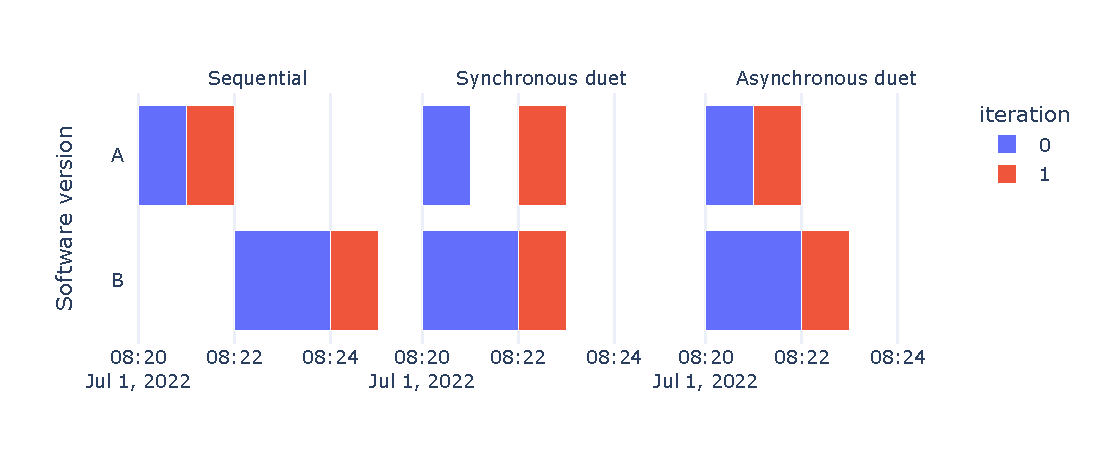
\includegraphics[width=.9\linewidth]{./figures/method_timeline.pdf}
	\caption{
	Comparison of different benchmarking methods sequential, synchronous duet, and asynchronous duet when comparing 2 software versions A and B.
	Benchmark runs 2 iterations with the same durations for all methods and versions.
	Note that version B introduced a regression where first iteration takes twice as long.
	X axes is an example timeline of measurements.
	}
	\label{fig:method_timeline}
\end{figure}

% RQ1 Runtime reduction
This example has the durations of iterations equal for all methods, that illustrates one immediate benefit of running duet benchmarks --- overall runtime reduction.
Ideally duet method could save up to $50\%$ or execution run time and hence halve execution costs.
However, in order to achieve such speedup, workloads running in parallel must not interfere with each other.

\begin{quote}
	\textbf{RQ1:} \emph{What are the runtime savings of duet methods compared to the sequential method?}
\end{quote}

% Mutual interference
To address mutual workload interference,~\citet{bulej2020duet} set up measurements in such a way that each benchmark was restricted to single dedicated virtual core.
Even then, it may be the case that the two virtual cores map to the same hardware threads of the same physical core.
Such virtual cores would then compete for the single shared physical core.
Here~\citet{bulej2019initial} rely on workload symetry which states that if a cloud were to exhibit systematic performance difference between the two virtual cores running duet workloads, it would likely exhibit similar unwarranted performance difference in other common concurrent workloads, such behavior would be likely considered a bug and remedied.
In other words they rely on fair CPU scheduling to work out mutual interference.
\citet{bulej2019initial} also note that this works only for similar workloads, which can be expected of neighboring commits or versions of the same software.

% External interference, Synchronized interference, Impact symetry for seqn syncduet and async duet.

\section{Synchronous vs. Asynchronous duet}

% Impact symetry on asynchronous duet
\Cref{fig:method_timeline} also note that synchronized duet methods are not always running in parallel.
Once an iteration finishes it has to wait for its pair iteration to finish, until then, this pair iteration runs alone.
It might seem that asynchronous duet solves this issue because iterations are not blocked on barrier, so the only iteration running alone will be the last iteration of either A or B, whichever finishes last.

However, asynchronous duet might be worse of in terms of equal impact symetry on parallel workloads due to ways benchmark harnesses and benchmarks themselves work.
\Cref{alg:harness} is a generic example of how inner loop of benchmark harness might look like.
Pre and post iteration functions might do some environment checks like running garbage collection or recording results.
Benchmark harness authors did not have any reason to care of reduced noise around the measured code, nor keep the loop tight.
Therefore it is natural that  asynchronous duet might suffer from this.

\begin{algorithm}
\begin{algorithmic}
	\Function{RunHarness}{$b$}
		\State \Call{Setup}{$b$}
		\For{$i \in 1 \dots I$}
		 	\State \Call{PreIteration}{}
			\State $start \gets$ \Call{clock.now}{}
			\State \Call{RunBenchmark}($b$)
			\State $end \gets$ \Call{clock.now}{}
			\State \Call{PostIteration}{$b$, $i$, $start$, $end$}
		\EndFor
		\State \Call{ValidateResults}{$b$}
		\State \Call{Teardown}{$b$}
	\EndFunction
\end{algorithmic}
\caption{
	Generic workings of the benchmark harness which executes a benchmark.
	Note that not all harnesses follow this structure --- some functions might be effectively empty.
	Specifically for synchronous duet~\citet{bulej2020duet} had to modify \emph{PreIteration} to wait on barrier.
}
\label{alg:harness}
\end{algorithm}

\Cref{fig:overlap_timeline} figure shows what implications can absence of synchronization have on workload overlaps.
With enough iterations, harness specifics, and potentially different A/B performance it is inevitable that workloads will diverge.
Even if workloads are partially overlapping, start of a workload might do different things, for example be CPU bound, compared to the end of the workload, that might be I/O bound.
This further hinders the impact symetry for asynchronous duet that synchronous duet method relies on.

% RQ2 Overlaps
\begin{quote}
	\textbf{RQ2:} \emph{How do workloads overlap in asynchronous duet?}
\end{quote}

\begin{figure}
	\centering
	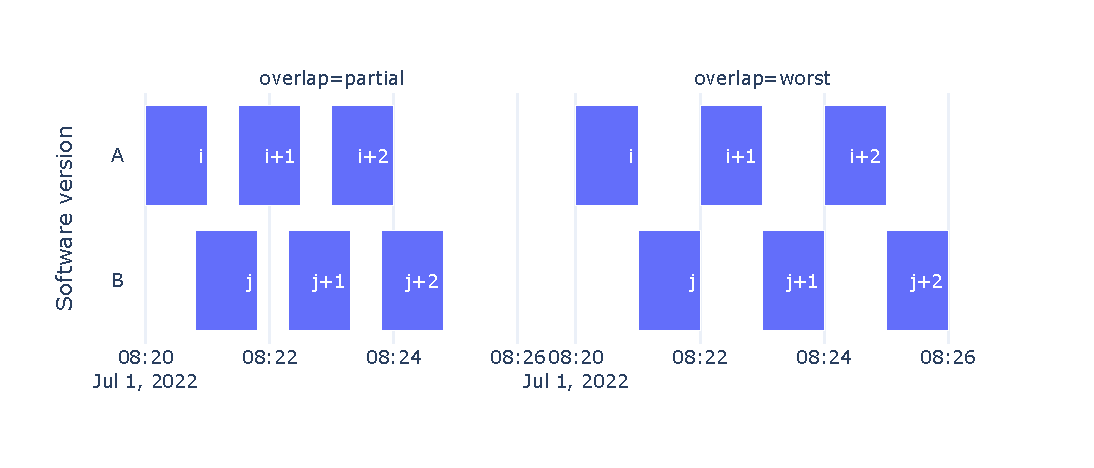
\includegraphics[width=.9\linewidth]{./figures/overlap_timeline.pdf}
	\caption{
		Tailored examples of how lack of synchronization might affect overlap of timed benchmark code.
		This is an example timeline of iterations of an \emph{asynchronous duet} measurement from an iteration $i$ and $j$ for versions $A$ and $B$ respectively.
		Focus on how versions $A$ and $B$ overlap --- just partially or even not at all.
	}
	\label{fig:overlap_timeline}
\end{figure}

For asynchronous duet method to be any useful runtime reduction and overlapping workloads are not enough.
Asynchronous duet method has to show variance improvements on par with the synchronized duet method.

% RQ3 Variable environment
\begin{quote}
	\textbf{RQ3:} \emph{What is the variance of asynchronous-duet compared to synchronous duet and sequential execution across different envrironments?}
\end{quote}

Additionally using similar approach to~\citet{laaber2019software} asynchronous and synchronous duet methods can be compared with sequential measurements in terms of \emph{minimal detectable slowdowns}~\xxx{cref to chap4}.

% RQ4 Minimal detectable slowdown
\begin{quote}
	\textbf{RQ4:} \emph{What are the minimal detectable slowdowns that we can detect with $95\%$ confidence?}
\end{quote}

% Why is it important - runtime reduction, variable environment, no suite modification
To summarize research into duet methods in this thesis focuses on:
\begin{description}
	\item[Runtime and Cost reduction] Duet methods have potential to drastically reduce, up to $50\%$, the execution time of benchmarks.
	\item[Accuracy] Synchronized duet method can reduce variance of benchmark results measured in variable environment, such as public cloud~\citet{bulej2020duet}. Question is if asynchronous duet can do the same?
	\item[Accesibility] Asynchronous duet relaxes synchronized requirement on benchmark harnesses which makes this method more broadly usable.
\end{description}
